% This template is kept quite simple in order to maintain the possibility of
% merging different documents using this particular template into a single
% volume. Please do not change the following layouting options.
\documentclass[
  a4paper,               % a4 paper
  twoside,               % two sided
  headings=small,        % chapter and section headings are smaller
  DIV=12,                % use a 12 part division of paper
  BCOR=1cm,              % use 1cm correction for binding
  headinclude=true,      % include header inside typearea
  footinclude=true,      % include footer inside typearea
  numbers=noenddot,      % no full stop after after last number of titles
  11pt]{scrartcl}        % 11 point article

\usepackage[T1]{fontenc}
\usepackage[utf8]{inputenc}
\usepackage[english]{babel}
\usepackage{palatino}
\usepackage{graphicx}
\usepackage{caption}
\fontfamily{ppl}
\selectfont
\pagestyle{empty}
\usepackage{setspace}
\setlength{\parindent}{0ex}
\setlength{\parskip}{0.5em}
\usepackage{url}
\usepackage{hyperref}
\usepackage{listings}


% You may add additional libraries here, but please do not mix up the layout.

\usepackage{graphicx}
\usepackage{tikz}



\lstset{% 
numbers=left, numberfirstline=true
}%
\begin{document}

\begin{center}
\emph{\huge Web Servers} \\[1em]
Markus Richter (\url{richter@informatik.uni-luebeck.de})
\end{center}

% \tableofcontents

\section*{Abstract}

Websites play an important part in the Internet, as they are used by millions of people every day world wide, thus this part of the Internet is called \emph{World Wide Web} or, for short, \emph{WWW} or \emph{Web}. In fact many people mean the WWW when they are speaking of the Internet. The WWW is build upon a huge net of Web servers which forms the basic structure of the Web. They provide support for essential technologies that make Web sites comfortable, interactive and attractive. This article focuses on those technologies which are used by servers in order to make appealing and modern Web sites possible. Furthermore, attention will be paid to the research results concerning performance improvements of Web servers by applying the scheduling policy called \emph{Shortest-Remaining-Processing-Time} (\emph{SRPT}), \emph{Least-Attained-Service}
(\emph{LAS}) and \emph{Preempt-On-Wait} (\emph{POW}).


\section{Introduction}
% The structure of the paper will be as follows. First it is important to make clear what the topic means, therefore an explanation to the term Web server will be provided. The core aspect of this paper, still, is its influence on Web development in particular and the quality of the Web in general and whether a Web server can assure it. So additionally a definition for a good and modern Website plus an explanation for Quality of Service (QoS) is needed and thus will also be presented. After that follows a brief history in order to put this paper in the right context. As moving on to more precise technology the basic concept of a Web server will be illustrated. Unfortunately, this concept alone as a toolbox is not enough to meet the criteria of a good and modern Web site, as we call it. Thus the toolbox need to be extended with more technologies (PHP, Java...) which will be introduced and explained. Then, the three most widely used Web servers providing the needed set of tools --- the \emph{Apache Web Server}, \emph{Tomcat} and the \emph{Internet Information Services (IIS)} --- will be introduced. In the final step possible answers to the previously mentioned questions will be given and explained.

The Internet not only grows larger every day, it also becomes more important and present in nearly every aspect of modern life. Nowadays it is not simply used for information gain between a few exclusive participants as it was initially intended but instead it is a platform for the purpose of communication, business and entertainment for millions of people. Those services, accessed through Web sites, ranging from browser games to e-commerce and online banking, are the key to the success of the Internet. \smallskip

The astonishing increase in numbers and functionality is made possible not least due to the use of Web servers. Inhomogeneous technologies like \textit{PHP} or \textit{Java Servlet} and \textit{JavaServer Pages} used to implement dynamic behaviour combined with static behaviour and international standards like \textit{HTTP} are being combined and hidden inside the Web servers and being presented as one solution. \smallskip

So as Web servers are playing such an important role for the internet in general and for Web sites in particular, the questions arise how they can support the development of Web sites towards more attractive and modern Web sites and additionally assure high performance in the Web. To answer this questions we will analyse the functionality behind a Web server which is needed to fulfil those needs. Furthermore we will take a close look at some methods and solutions in order to increase the performance.

\subsection{Definitions}

First it is essential to define and explain the terminology being used in order to build up an initial understanding of Web servers and the essential technologies associated with them. 

\subsubsection{Web server}
The term Web server is being used to describe hardware as well as software. In the first case the computer is meant on which a Web site is hosted, in the second case the program that runs on the computer. Being part of the \textit{Server Client Architecture} the Web server basically takes \textit{HTTP} request from clients and answers with \textit{HTTP} responses. 

\begin{figure}[h]
  \centerline{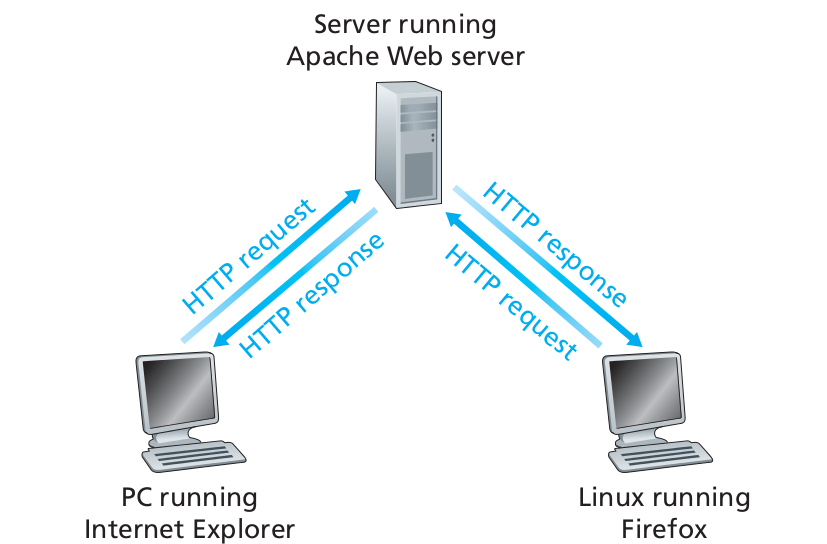
\includegraphics[width=8cm]{pics/client_server.png}}
  \caption{Client Server Architecture.\\Taken from \cite{kurose}}
\end{figure}

\subsubsection{HTTP}
The \emph{HyperText Transfer Protocol} (\textit{HTTP}) is an \textit{application-layer} protocol that controls the exchange between client and server. It is defined in \cite{rfc1945} and \cite{rfc2616}. \textit{HTTP} is divided in two parts: a client and a server program. Those two parts communicate with each other by using \textit{HTTP} messages \cite{kurose}. 

\subsubsection{Web site}
A Web site consists of one or many Web pages, also called \textit{documents}. A Web page contains objects which are files. Those files can be \textit{HTML files, images, Java applets} etc. Each object is addressed by an \emph{URL} --- \emph{Uniform Resource Locator}. In most cases the Web site has a base \textit{HTML} file which references many different objects \cite{kurose}. We speak of an \textit{attractive} and \textit{modern} Web site if it is in line with expectations regarding \textit{appearance, security, performance and interactivity}. 

\subsection{Concept}
The concept of a Web server is based mainly on \textit{HTTP}. As mentioned before \textit{HTTP} consists of a client and a server program. The client program is in most cases a \textit{Web browser} while the server program is the Web server itself. The communication between those two programs is reduced to the \textit{HTTP} methods \emph{GET, POST, HEAD, PUT,} and \emph{DELETE}. In the majority of cases the GET method is being used, namely when the client requests a file. The request is then answered by the server with a response containing meta data and the payload itself. This concept is simple but completely sufficient and has proved successful over the years. \textit{HTML} is a descriptive language used for visualisation only and is static, hence, contains no logic and therefore is not a programming language.\\
In order to enable \textit{dynamic} Web sites the Web server can generate --- by using \textit{server-side technologies} --- those \textit{HTML} files each time an interaction appears, e.g. if the current date needs to appear at the Web site. So the client constantly gets changed static \textit{HTML} files what simulates dynamic behaviour. From the view of the client it seems like the current \textit{HTML} file is changing dynamically but in reality the server keeps responding with new adjusted \textit{HTML} files.\\
\autoref{fig-webserverconcept} illustrates  that almost all responsibility for creating and manipulating content is capsuled inside the Web server, although there are technologies used which allow execution of code on the client side. 

\begin{figure}[h]
  \centerline{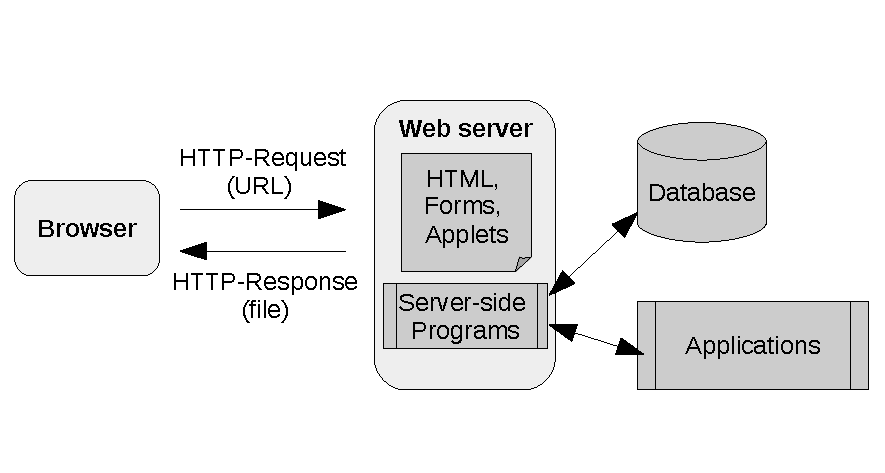
\includegraphics[width=10cm]{pics/webclient.pdf}}
  \caption{Concept of an HTTP Web server}
  \label{fig-webserverconcept}
\end{figure}

\subsection{History}
% After the USSR launched Sputnik in 1957 the US were forced to face the new possibilities for global telecommunications and even more the danger of a nuclear attack from the outer space. In response, the US established the Advanced Research Projects Agency (ARPA) to build up US lead in science and technology relevant to the military. As a consequence the Packet-switching networks were developed which could withstand large scale destruction due to many different routes a package could take. In 1969 ARPANET was commissioned what was the birth of the Internet. Initially it was a closed network with a few nodes --- mainly universities --- but as time passed more and more services like E-mail were invented and even more networks were founded. Nonetheless, the earlier internet were a set of disconnected networks. 

The history of Web server is closely tied to the history of the Internet. But even though the internet kept growing rapidly since \emph{ARPANET} was established in the nineteen sixties, its size and popularity was not even close to what it is today until the most important development for the Internet to date was accomplished: In 1991 \emph{CERN} released the \emph{World Wide Web} developed by Tim Berners-Lee \cite{webhistory}. With it came the first \textit{HTTP} Web server: The CERN httpd which worked with \textit{HTTP} and \textit{HTML}\cite{cernHttpd}. Until now this principle has not changed significantly. In spite of relying on this principle which only provides static content in the form of \textit{HTML} files there is still dynamic behaviour in the web. This advantage is only possible thanks to server-side technologies like \textit{CGI}, \textit{JSP} or \textit{PHP}. 

\section{Server-side Technologies}

\autoref{fig-webserverconcept} already indicates a functionality not intended in former Web servers (server-side programs, database, applications). As the Web grew, the need for interactivity became more urgent. As a result a number of competing technologies evolved to satisfy those needs for attractive and modern Web sites. All technologies have in common that they are not integrated in the Web server core program but act as an external program or as module located at the same machine the Web server program is running on, hence, on the Web server's hardware. Although \cite{w3TechsStats} reveals, that Java based technology \textit{JSP} is used least often than \textit{ASP.NET}, we will concentrate on \textit{PHP} and \textit{JSP} only, because they are not limited to proprietary platforms. 

\subsection{Common Gateway Interface}
In \cite{cgiSpecs} \textit{CGI} is defined as "a simple interface for running external programs, software or gateways under an information server in a platform-independent manner". \autoref{fig-cgi} illustrates the functionality of \textit{CGI}.\cite{gundavaram1996cgi} describes it fairly well. Usually the client requests a \textit{CGI} program the same way it requests any other Web document by using the \textit{HTTP GET Method}. The difference is that the server --- provided that it implements the \textit{CGI specifications} --- tries to execute the program.  \autoref{lst:cgiProgram} shows an example of how such a GET method can look like. All the information, like e.g. the data formats the client accepts, are made available to the \textit{CGI} program via input by using the \textit{standard input}, e.g. STDIN on UNIX systems and from UNIX environment variables. The result of the execution can either be a new document or an \textit{URL} to an existing one. It is then passed on the Web server via \textit{standard output} (STDOUT) as a data stream. Like the definition mentions, \textit{CGI} is platform-independent which also means it is not limited to certain programming languages, thus, the CGI program or script can be implemented in different ones.\\
A significant disadvantage of \textit{CGI} is its low scalability and bad performance as it forces the operating system to fork an own process for each \textit{HTTP} request, resulting in high overhead \cite{brittain2007tomcat}. Because of this, modern Web servers provide their own, more performant, solutions for popular technologies, e.g. \textit{mod\_php} or \textit{mod\_perl} modules for \textit{Apache} \cite{welling2008php}, so \textit{CGI} is barely used nowadays. 

\begin{lstlisting}[captionpos=b,caption={Client request for CGI program. Taken from \cite{gundavaram1996cgi}},label=lst:cgiProgram]
GET /cgi-bin/welcome.pl HTTP/1.0
Accept: www/source
Accept: text/html
Accept: image/gif
User-Agent: Lynx/2.4 libwww/2.14
From: shishir@bu.edu
\end{lstlisting}

\begin{figure}[h]
  \centerline{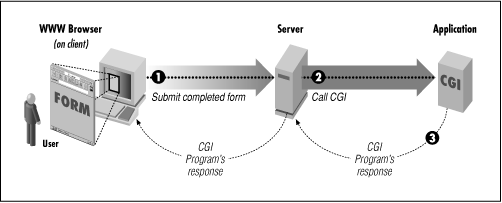
\includegraphics[width=10cm]{pics/cgi.png}}
  \caption{How CGI works. Taken from \cite{gundavaram1996cgi}}
  \label{fig-cgi}
\end{figure}

\subsection{PHP:Hypertext Preprocessor}

\emph{PHP} stands for \emph{PHP:Hypertext Preprocessor}, thus it is a recursive acronym \cite{PHPPreface}. \cite{PHPPreface} defines it as "a widely-used Open Source general-purpose scripting language that is especially suited for Web development and can be embedded into \textit{HTML}. Its syntax draws upon \textit{C}, \textit{Java}, and \textit{Perl}, and is easy to learn." Because of the fact, that \textit{PHP} is a scripting language it needs to be interpreted. The interpreter can either be a module or a separate \textit{CGI} binary, although the module version is usually being used due to performance reasons \cite{welling2008php}. \textit{PHP} is relatively easy and straight-forward because, as illustrated in \autoref{lst:php}, it can be embedded inside \textit{HTML} files and executed every time the \textit{HTML} file is accessed, generating \textit{HTML} or other output relevant for the visitor \cite{welling2008php}. This way dynamic behaviour is achieved.\\
According to \cite{w3TechsStats}, \textit{PHP} is by far the most popular used technology in Web development. The reasons are, amongst others, high performance, scalability, object-oriented support, database integration and low costs. It is also often combined with \textit{MySQL}, an open-source relational database management system. On the other hand, \cite{bowen2002apache} mentions some drawbacks, e.g. the code maintenance, that can be made difficult easily by potential lacking of structure due to mixing up of \textit{HTML} and \textit{PHP} code. Also \textit{PHP} is not fully object-oriented, because some object-oriented capabilities like private variables, multiple inheritance are missing. Furthermore, it has some problems with stability and interdependences, because \textit{PHP} usually relies on external libraries, e.g. for database connectivity, which may be on different stages of development. \textit{PHP} is usually used together with \textit{Linux}, \textit{Apache Web server} and, as mentioned, \textit{MySQL}, forming the well known \textit{LAMP architecture}. 


\begin{lstlisting}[language=php, captionpos=b,caption={PHP embedded in HTML. Taken from \cite{welling2008php}},label=lst:php]
<?php
echo "<p>Order processed at ";
echo date('H:i, jS F Y');
echo "</p>";
?>

\end{lstlisting}

\subsection{JavaServer Pages}

\emph{JavaServer Pages} (\emph{JSP}) is similar to \textit{PHP}, but instead it is easier to achieve more structure and it uses \textit{Java} as programming language. Although \textit{JSP} can be used independently it is meant to be viewed in a \textit{MVC} design fashion \cite{downey2008web}. \autoref{fig-jspMvc} illustrates such an architecture.\\
This means that \textit{JavaBeans} encapsulates the data and additionally the methods which work on it. The \textit{servlet} is the controller that gets the request and sends back the responses to the Web server. The \textit{JSPs} are responsible for the view. Similarly to \textit{PHP}, \textit{JSPs} are \textit{HTML} files with embedded Java code, but which usually are directives to display data from the model, not logic.\\
\autoref{lst:jsp} shows a simple case, where the \textit{JSP} uses a \textit{JavaBean} called refData to access the parameters from the \textit{HTTP} \textit{request}. Before that, the \textit{servlet} (controller) has to add the bean to the session.\\
All this is wrapped inside a container. A container is needed for communication between the JSP technology and the Web server. Furthermore it handles the lifecycle management of servlets, multithreading support and security \cite{downey2008web}. A container, which is very popular today, is for example, \textit{Tomcat} that is based on the \textit{Apache Web server}.

\begin{figure}[h]
  \centerline{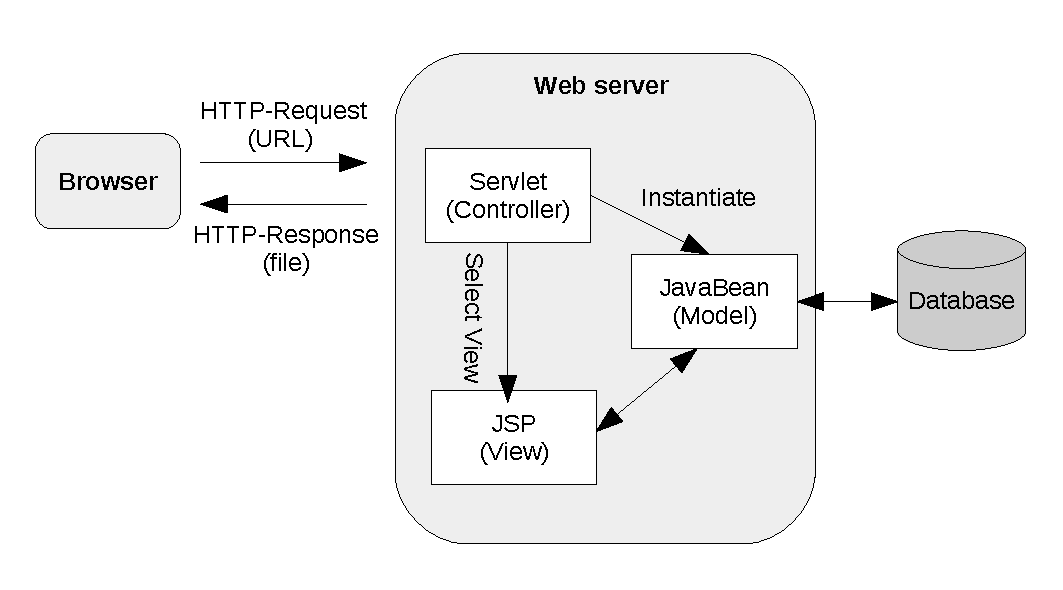
\includegraphics[width=12cm]{pics/jspMVC.pdf}}
  \caption{Model of JSP}
  \label{fig-jspMvc}
\end{figure}

\begin{lstlisting}[language=html, captionpos=b,caption={Java embedded in HTML. Taken from \cite{downey2008web}},label=lst:jsp]
Hobby:
<input type="text" name="hobby" value="${refData.hobby}">
<br>
Aversion:
<input type="text" name="aversion" value="${refData.aversion}">

\end{lstlisting}

\section{Increasing Performance}

The number of Web users grows strongly, but as expanding the Web infrastructure is expensive other solutions have to be found in order to maintain, or even increase the performance of the Web. One possible solution, that Web server can participate in, is size-based scheduling proposed by \cite{schroederSize} and \cite{schorederSchedule}. Their work shows that, by simply changing the order in which request being scheduled, the expected response time of every \textit{HTTP request} can be reduced. Most traditional Web server use a \textit{fair} scheduling policy, which means "that the Web server proportions its resources fairly among those requests ready to receive service" \cite{schroederSize}. So the new approach is now to use \textit{unfair} scheduling: Priority is given for short request or those requests with short remaining file size. This approach goes along with the well-known scheduling algorithm \emph{preemptive Shortest-Remaining-Processing-Time-first} (\emph{SRPT}).\\
\autoref{fig-srpt} shows the results of an implementation using \textit{SRPT} scheduling. An Apache Web server and a Linux operation system was used. In order to adjust the scheduling, implementation had to be done at kernel level. The left figure shows that the mean response time of the Web server using the \textit{SRPT} approach is significantly lower compared to the Web server working with the default fair scheduling policy. The performance benefits of \textit{SRPT} even increases dramatically as the server load gets higher. The right figure shows for both approaches the response time as a function of the request size. It can be seen that for 99\% of file sizes \textit{SRPT} is performing much better and large file sizes belonging to the other 1\% are only penalised minimally, which means both response times are either nearly identical or for the very largest files \textit{SRPT} results in 5\% larger response time.\\
Although this results are convincing there are still reservations against \textit{SRPT}. Mostly, it is the fear that big jobs will "starve" \cite{schorederSchedule}. Thus, \cite{schorederSchedule} argues that web file sizes exhibit highly variable statistical distributions with heavy-tails and that for those highly variable distributions \textit{SRPT} does not unfairly penalise long jobs. Additionally, \cite{schorederSchedule} show that \textit{SRPT}-based scheduling is also able to minimise the number of connections at a server "by always working on the connection with the smallest amount of work left" \cite{schorederSchedule} and, hence, can help to face the problem of transient periods of overload.\\
\textit{SRPT} therefore is a promising approach for \textit{HTTP requests}, but that means it only can achieve a performance boost with static files, as \textit{HTTP requests}, e.g. using the GET method, concerns physical files like images or \textit{HTML} files. In order to increase performance of dynamic content processing we have to look at the common bottleneck in processing dynamic web requests which is the database backend \cite{McWherter}. This makes it more complicated to apply the \textit{SRPT} approach on dynamic content for two reasons.  First, for \textit{SRPT} it is essential to know the length of a transaction before execution. \cite{schorederSchedule} present a preemptive policy called \emph{Least-Attained-Service} (\emph{LAS}) for systems where size estimation is not possible, like for example in scheduling in routers. \textit{LAS} guesses the remaining service time of a job based on the service it has received so far. This way, \textit{LAS} converges towards \textit{SRPT} behaviour.\\
Given that, the second problem is that existing database management systems do not support effective transaction prioritisation for web-based transacional workloads. This means they are often lock-bound and thus need lock scheduling \cite{McWherter}. Basically, databases lock to protect shared resources like tables, data rows etc.\\
\cite{Callison09} provides more detailed information about locks. \cite{McWherter} propose a policy called \emph{Preempt-On-Wait} (\emph{POW}). The algorithm preempts low-priority transactions in favour of high-priority transactions, but if and only if the low-priority transaction currently, or in the future, waits for some other lock. By doing this it is guaranteed that already partially completed work will not be lost. \autoref{fig-pow} shows the response time of \textit{POW} compared to \textit{standard} --- transactions are not prioritised --- and two other related policies \textit{PAbort} and \textit{NPrioinher}. \textit{PAbort} stands for Preemptive Abort. In that case, a low-priority transaction which blocks a high-priority one is always immediately preempted, what causes overhead caused by rolling back and restarting. \textit{NPrionher} on the other hand grands low-priority transactions that block high-priority ones temporarily high priority to release locks more quickly. This causes worse high priority performance as low priority transactions need to be finished first. \textit{POW}, therefore, is a compromise of both. Given that, \textit{POW} improves mean response time of high priority transactions by a factor of 8, while only increasing the mean response time of low priority ones by less than 10\% \cite{schorederSchedule}. Combined with \textit{SRPT} scheduling for static content, both, \textit{POW} and \textit{SRPT}, form a appealing solution for increasing performance of Web servers and thus of the Web. 




\begin{figure}[h]
\centerline{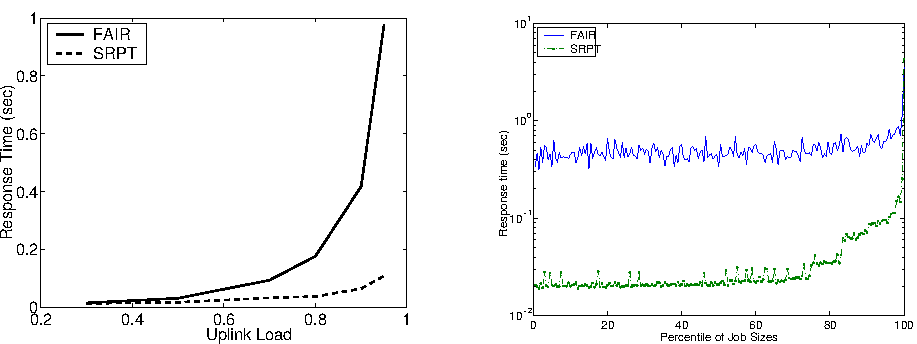
\includegraphics[width=15cm]{pics/srpt.pdf}}
\caption{(Left) Shows the improvement in mean response time of \textit{SRPT} scheduling over \textit{FAIR} scheduling for static requests at a web
server in a LAN setting. (Right) Shows mean response time as a function of the size of the requested file, where system load is fixed at
$\rho$ = 0.8. Taken from \cite{schorederSchedule}}
\label{fig-srpt}
\end{figure}

\begin{figure}[h]
\centerline{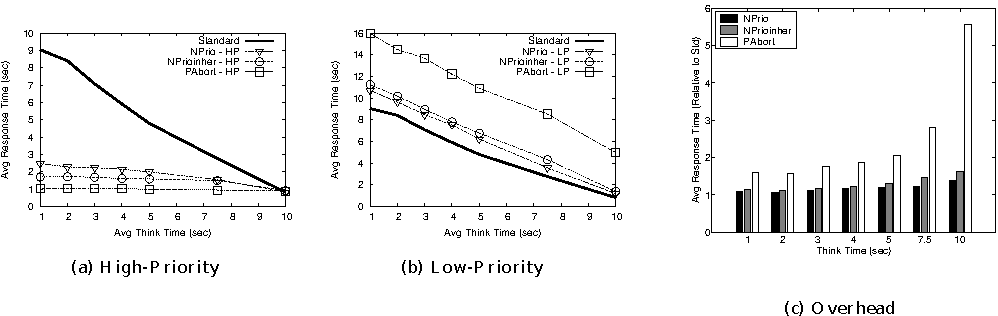
\includegraphics[width=15cm]{pics/pow.pdf}}
\caption{Average response time for high- and low-priority transactions for \textit{POW}, \textit{PAbort}, and \textit{NPrioinher} as a function of load (a) and (b). Aggregate high- and low-priority average response time
relative to \textit{Standard} (c). Taken from \cite{McWherter}
}
\label{fig-pow}
\end{figure}

\section{Conclusions}
In this article, we have defined what is essential for today's Web server and introduced some popular technologies. We started with a brief explanation of the basic principles of a Web server which have not changed much since 1991. We saw, that those principles were usually intended for static content and still, despite of this limitations, modern Web server provide dynamic content. We showed that this is due to innovative server-side technologies like \textit{PHP} or \textit{JSP}. Although today's Web servers are powerful, we also argued, that there is still space for improvements, especially when it comes to performance. Consequently, we looked at some promising solutions being in research and showed that they can help and how they can help.


\bibliographystyle{apalike}
\bibliography{ref}

\end{document}
